\documentclass[pscyr,nonums]{hedlab}
\usepackage[russian]{babel}
\usepackage[utf8]{inputenc}
\usepackage{graphicx}
\usepackage{listings}

\graphicspath{{images//}}

\labnum{3}
\labname{Метод симуляции отжига.}
\student{Голубев А.~В.}
\labdate{}

\begin{document}
    \makeheader
    \lstset{language=c++, basicstyle=\tiny}

    \noindent\emph{Цель работы:} 
    \begin{enumerate}
        \item познакомится c методом симуляции отжига;
        \item реализовать алгоритм на языке программирования;
        \item получить значения минимума функции на некоторых входных данных.
    \end{enumerate}

    В качестве исследуемой функции выбрана:
    \[
        f(x, y) = x^4 + y^3 + x^2 + y
    \]

    График исследуемой функции:
    \begin{figure}[h!]
        \centering
        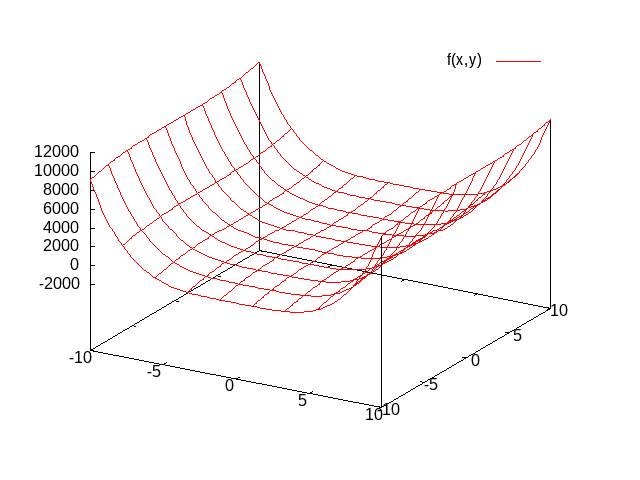
\includegraphics[width=.47\textwidth]{graph}
    \end{figure}

    Полученные результаты:
    \begin{center}
        \begin{tabular}{|c|c|c|c|c|c|}
            \hline
            R, размер поля & N, количество иттераций & T, температура & 
            x & y & f(x, y) \\ \hline
            10.0 & \( 10^3 \) &  30.0 &  0.553807 &  1.645520 &  6.501920 \\ \hline
             5.0 & \( 10^5 \) & 100.0 &  0.018133 & -0.879679 & -1.560080 \\ \hline
             5.0 & \( 10^6 \) & 100.0 &  0.696922 & -0.603472 & -0.101640 \\ \hline
             1.0 & \( 10^6 \) & 100.0 &  0.139441 & -0.027213 & -0.007410 \\ \hline
             1.0 & \( 10^6 \) & 500.0 &  0.049215 &  0.011560 &  0.013989 \\ \hline
             1.0 & \( 10^8 \) & 500.0 & -0.008203 & -0.347439 & -0.389313 \\ \hline
        \end{tabular}
    \end{center}

    \clearpage

    \noindent Исходный код программы
    \lstinputlisting{annealing.cpp}
\end{document}
